% Beamer do material do curso de Verão (2015) do IME-USP
% Introdução ao Projeto de Jogos
%
% Baseado no template LaTeX das apresentações do LIDET versão 2
% (https://github.com/luigivieira/LIDET)
%

\providecommand\classopts{}
\expandafter\documentclass\expandafter[table, usenames, svgnames, dvipsnames,%
                                       \classopts]{beamer}
\usepackage{etex}
\usepackage{beamerthemeshadow}
\usepackage[portuguese]{babel}
\usepackage[utf8]{inputenc}
\usepackage[absolute,overlay]{textpos}
\usepackage{array}
\usepackage{framed}
\usepackage{booktabs}
\usepackage[compatibility=false]{caption}
\usepackage{subcaption}
\usepackage{outlines}
\usepackage{ulem}
\usepackage{xcolor,colortbl}
\usepackage{ragged2e}
\usepackage{tikz}

% ---------------------------------------------------------------------------- %
% Presentation definitions
% ---------------------------------------------------------------------------- %
\usetheme{Luebeck}
\hypersetup{pdfpagemode=FullScreen} % Starts the presentation in full screen

% layout
\setbeamerfont{frametitle}{size=\normalsize}
\setbeamerfont{title}{size=\normalsize}
\beamertemplatenavigationsymbolsempty
\setbeamertemplate{bibliography item}[text]%
\setbeamertemplate{headline}{} % Remove a barra superior.

% colors
\definecolor{lidet_orange}{rgb}{0.9, 0.49, 0.09}
\definecolor{lidet_black}{rgb}{0.2, 0.2, 0.2}

\setbeamercolor{title}{bg=lidet_orange}
\setbeamercolor{structure}{bg=white, fg=lidet_orange}
\setbeamercolor{normal text}{fg=black}
\setbeamercolor{section in head/foot}{fg=white, bg=lidet_black}
\setbeamercolor{postit}{fg=white, bg=lidet_orange!90!lidet_black}

% shadow
\makeatletter
\pgfdeclareverticalshading[black,bg]{bmb@shadow}{200cm}{%
    color(0bp)=(lidet_black!25);%
    color(4bp)=(black!50!bg);%
    color(8bp)=(black!50!bg)%
}
\pgfdeclareradialshading[black,bg]{bmb@shadowball}{\pgfpointorigin}{%
    color(0bp)=(black!50!bg); color(4bp)=(lidet_black!25)%
}
\pgfdeclareradialshading[black,bg]{bmb@shadowballlarge}{\pgfpointorigin}{%
    color(0bp)=(black!50!bg);%
    color(4bp)=(black!50!bg);%
    color(8bp)=(lidet_black!25)%
}
\makeatother

% Captions for images and tables
\setlength{\abovecaptionskip}{5pt plus 5pt minus 5pt}
\setlength{\belowcaptionskip}{5pt plus 5pt minus 5pt}
\captionsetup[figure]{font=scriptsize,labelfont=scriptsize}
\captionsetup[table]{font=scriptsize,labelfont=scriptsize}
\captionsetup{labelformat=empty,labelsep=none}

% Dimensions for table rules
\setlength\heavyrulewidth{0.1em} 
\setlength\lightrulewidth{0.01em}
\setlength\belowrulesep{0.10ex}
\setlength\aboverulesep{0.10ex}

% Define macros to mark the begining and ending of references
% Basically, handles the automatically spanned frames (due to parameter
% allowframebreaks)
% as backup frames, so they do not influence in the frame numbering
\newcommand{\referencesbegin}{
   \newcounter{framenumberappendix}
   \setcounter{framenumberappendix}{\value{framenumber}}
}
\newcommand{\referencesend}{
   \addtocounter{framenumberappendix}{-\value{framenumber}}
   \addtocounter{framenumber}{\value{framenumberappendix}} 
}

% Section frames (that appear before each section)
\AtBeginSection[] 
{
	{
        % Hide the footline locally for these frames
		\setbeamertemplate{footline}{}
		\begin{frame}<beamer>[noframenumbering]
			\begin{center}
				\begin{tikzpicture}
					\node[align=left, left color=lidet_orange,%
                          right color=lidet_orange, draw, rounded corners,%
                          minimum width=10cm, minimum height=1cm]%
                          {\color{white} \textbf{\insertsectionhead}};
				\end{tikzpicture}
			\end{center}
			\footnotesize{\tableofcontents[currentsection,%
                          hideothersubsections]}
		\end{frame}
	}
}

\DeclareGraphicsExtensions{.pdf,.jpg,.png}
\graphicspath{{./images/}}

% ---------------------------------------------------------------------------- %
% Presentation title, author and institution
% ---------------------------------------------------------------------------- %
\newcommand{\lessontitle}{Aula 3 - Pensando no gameplay}
\title{\textbf{Introdução ao Projeto de Jogos}}
\subtitle{{\small \lessontitle}}

\newcommand{\autores}{Luiz C. Vieira, Vinícius K. Daros}
\author[\autores]{\scriptsize
    Luiz Carlos Vieira e Vinícius Kiwi Daros\\
    \{luigivieira,vinicius.k.daros\}@gmail.com
}

\newcommand{\lidet}{LIDET (IME - USP)}
\institute[\lidet]{\\[1.0mm] 
Curso de Verão (2015)\\
Departamento de Ciência da Computação}

\date{{\tiny 13 de Janeiro de 2015}}

% ---------------------------------------------------------------------------- %
% Presentation content
% ---------------------------------------------------------------------------- %

% ---------------------------------------------------------------------------- %
\begin{document}
% ---------------------------------------------------------------------------- %

% ---------------------------------------------------------------------------- %
% First Slide (index 0) = cover
% ---------------------------------------------------------------------------- %

{%\usebackgroundtemplate{}} 
\begin{frame}[plain, noframenumbering]
	\begin{columns}[c]
		\column{0.2\textwidth}
			\hspace*{-1.5em}
			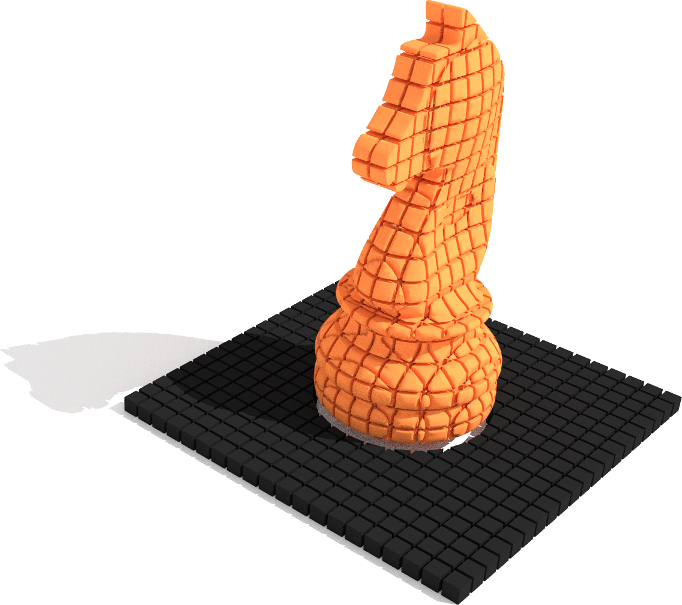
\includegraphics[width=0.35\paperwidth]{side_bar}\\
		\column{0.01\textwidth}
		\column{0.70\textwidth}
			\titlepage
			\hspace*{+0.5em}
			\begin{center}
				
\includegraphics[height=1.0cm]{lidet-logo}\\
				
\includegraphics[height=1.0cm]{ime-logo}\\
			\end{center}
	\end{columns}
	%\addtocounter{framenumber}{-1}
\end{frame}
}

% ---------------------------------------------------------------------------- %
% Other Slides (index from 1 onwards)
% ---------------------------------------------------------------------------- %

% setup navigation symbols and footline
\setbeamertemplate{navigation symbols}{}
\makeatletter
\setbeamertemplate{footline}{%
    \leavevmode%
    \hbox{%
        \begin{beamercolorbox}[wd=0.28\paperwidth,ht=4ex,dp=1ex,left,%
                               leftskip=2ex]{author in head/foot}%
            \usebeamerfont{title in head/foot}
            \insertdate\newline%
            \vskip 0.6ex%
            \autores
        \end{beamercolorbox}%
        \begin{beamercolorbox}[wd=0.53\paperwidth,ht=4ex,dp=1ex,center]%
                              {author in head/foot}%
            \usebeamerfont{author in head/foot}\lessontitle%
        \end{beamercolorbox}%
        \begin{beamercolorbox}[wd=0.19\paperwidth,ht=4ex,dp=1ex,right,%
                               rightskip=2ex]{author in head/foot}%
            \insertframenumber{}/\inserttotalframenumber \newline
            \lidet%
        \end{beamercolorbox}%
    }%
    \vskip 4cm%
}
\makeatother

% ---------------------------------------------------------------------------- %
\begin{frame}[plain]
\frametitle{\textbf{Agenda}}
	\hspace*{+4.0em}
	\footnotesize{ \tableofcontents }
\end{frame}


% ---------------------------------------------------------------------------- %
\section{Gameplay vs. Jogabilidade}
% ---------------------------------------------------------------------------- %

% ------------------------------
\begin{frame}{\textbf{Gameplay vs. Jogabilidade}}
    \centering
    \begin{minipage}{7cm}
        \begin{description}
            \item[Gameplay:] ações dentro do jogo
            \vskip 1cm%
            \item[Jogabilidade:] capacidade de jogar bem\\
                                 (usabilidade dentro do jogo)
        \end{description}
    \end{minipage}
\end{frame}


% ---------------------------------------------------------------------------- %
\section{CCC - Character (Personagem), Câmera, Controle}
% ---------------------------------------------------------------------------- %

% ------------------------------
\subsection{Character (personagem)}

% ------------------------------
\begin{frame}{\textbf{Character (personagem)}}
    \centering
    \begin{minipage}{7cm}
        \begin{itemize}
            \item Forma e função
            \vskip 1cm%
            \item Personalidade
        \end{itemize}
    \end{minipage}
\end{frame}

% %s/^zxzx\n\(.*\)\n\(.*\)\n\(.*\)\.png/\% ------------------------------\r\\begin{frame}{\\textbf{Círculos}}\r    \\centering\r    \\begin{figure}\r        \\includegraphics[height=5cm]{\3}\r        \\caption{\1\\footnote{\\url{\2}}}\r    \\end{figure}\r\\end{frame}/g
%zxzx
%Sonic
%http://www.powersonic.com.br/downloads/artworks/classicos/Sonic_3.png
%sonic.png
\begin{frame}{\textbf{Círculos}}
    \centering
        \begin{figure}%
            \begin{subfigure}{0.3\textwidth}%
                \centering
                
\includegraphics[height=5cm]{sonic}%
                \caption{Sonic\footnotemark{}}%
            \end{subfigure}%
            \begin{subfigure}{0.3\textwidth}%
                \centering
                
\includegraphics[height=5cm]{bomberman}%
                \caption{Bomberman\footnotemark{}}%
            \end{subfigure}%
            \begin{subfigure}{0.3\textwidth}%
                \centering
                
\includegraphics[height=5cm]{sackboy}
                \caption{Sackboy\footnotemark{}}%
            \end{subfigure}%
    \end{figure}
\footnotetext[1]{\url{http://www.powersonic.com.br/downloads/artworks/classicos/Sonic_3.png}}
\footnotetext[2]{\url{http://img2.wikia.nocookie.net/__cb20111012003236/bomberman/images/6/6d/Bomberman_Art_BSDS.jpg}}
\footnotetext{\url{http://vignette3.wikia.nocookie.net/sackisback/images/d/d6/Sackboy_sitting.png/revision/latest/scale-to-width/1000?cb=20140627233414}}
\end{frame}
% CÍRCULOS

% ------------------------------
\begin{frame}{\textbf{Círculos}}
    \centering
    Simplificando bastante, pode-se\\
    fazer um personagem assim:

    \begin{figure}
        
\includegraphics[height=5cm]{kirby}
        \caption{Kirby (Kirby's Return to Dream Land)\footnote{\url{http://upload.wikimedia.org/wikipedia/en/2/22/Kirby_Wii.png}}}
    \end{figure}
\end{frame}

% ------------------------------
\begin{frame}{\textbf{Círculos}}
    \centering
    Ou até assim:

    \begin{figure}
        
\includegraphics[height=4cm]{pacman}
        \caption{Pacman\footnote{\url{http://upload.wikimedia.org/wikipedia/commons/4/49/Pacman.svg}}}
    \end{figure}
\end{frame}

% TRIANGULAR
% ------------------------------
\begin{frame}{\textbf{Triângulo na cabeça}}
    \centering
    \begin{figure}
        
\includegraphics[height=5cm]{neo_cortex}
        \caption{Doctor Neo Cortex (Crash Bandicoot)\footnote{\url{http://i.ytimg.com/vi/z4JKaqVndYM/hqdefault.jpg}}}
    \end{figure}
\end{frame}

% ------------------------------
\begin{frame}{\textbf{Triângulo na cabeça}}
    \centering
    \begin{figure}
        
\includegraphics[height=5cm]{diablo}
        \caption{Diablo (Diablo III)\footnote{\url{http://diablo.incgamers.com/gallery/data/543/Diablo_Glowei009c.jpg}}}
    \end{figure}
\end{frame}

% ------------------------------
\begin{frame}{\textbf{Triângulo na cabeça}}
    \centering
    \begin{figure}
        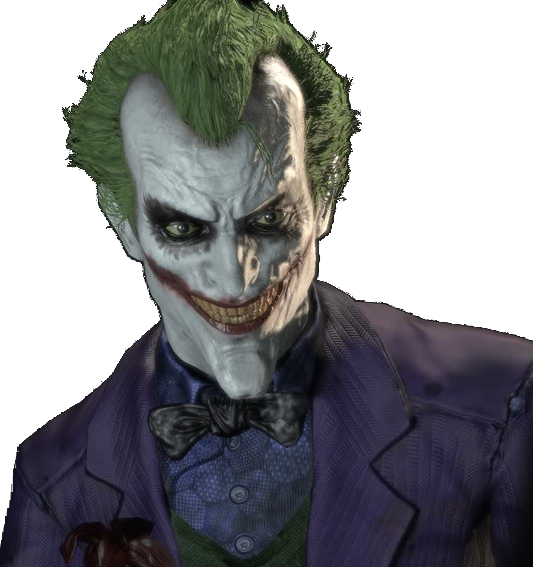
\includegraphics[height=5cm]{joker}
        \caption{Joker (Batman Arkhan Asylum)\footnote{\url{http://img.photobucket.com/albums/v299/Sepharih/Batman/Joker_1.jpg}}}
    \end{figure}
\end{frame}

% ------------------------------
\begin{frame}{\textbf{Triângulo na cabeça}}
    \centering
    \begin{figure}
        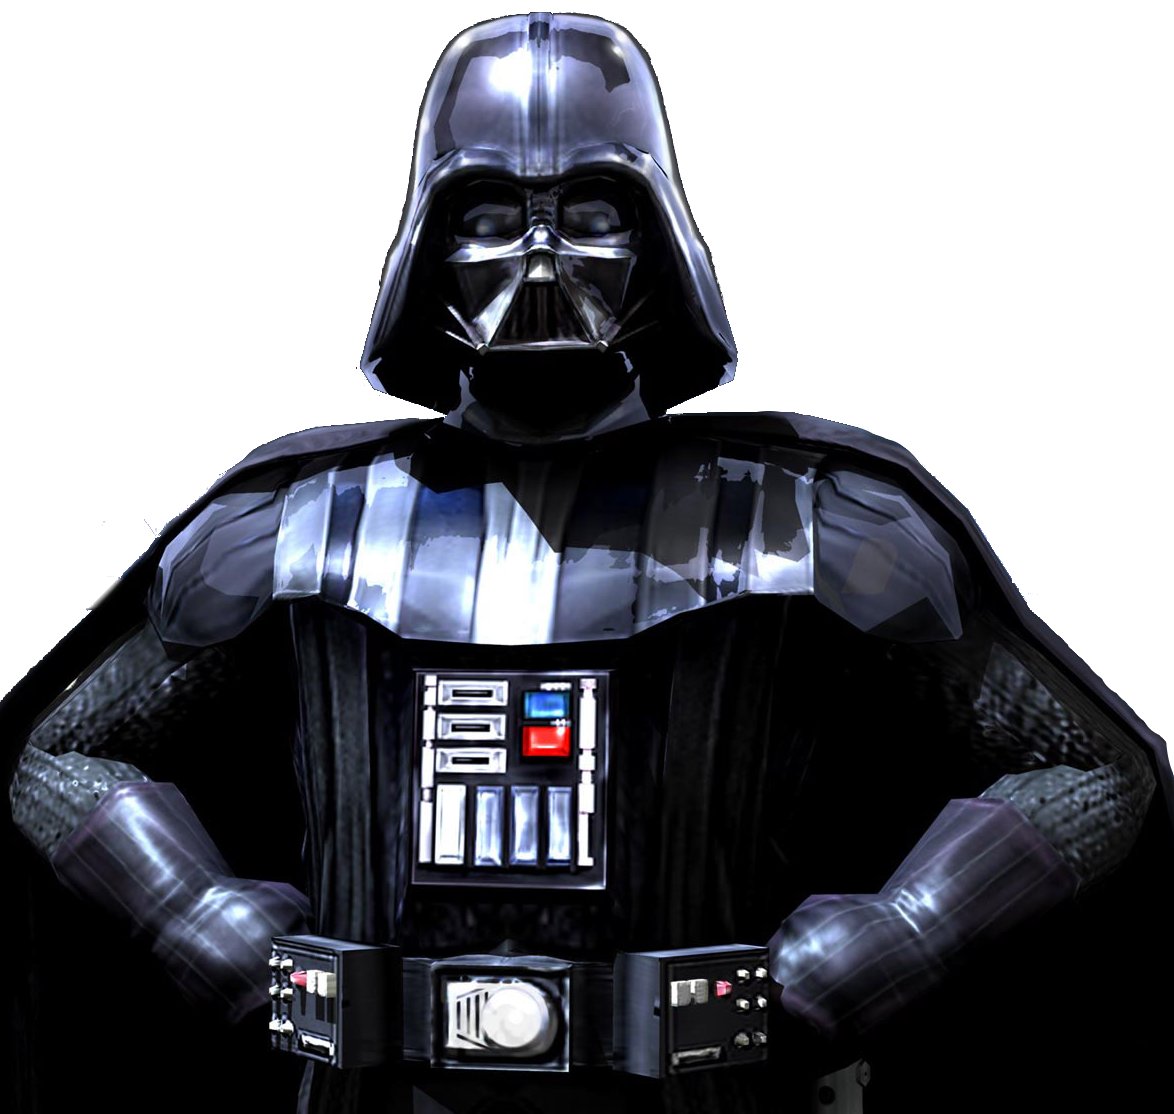
\includegraphics[height=5cm]{vader}
        \caption{Darth Vader (Star Wars)\footnote{\url{http://www.versusbattle.com/wp-content/uploads/2013/03/darth-vader.jpg}}}
    \end{figure}
\end{frame}

% ------------------------------
\begin{frame}{\textbf{Triângulo na cabeça}}
    \centering
    \begin{figure}
        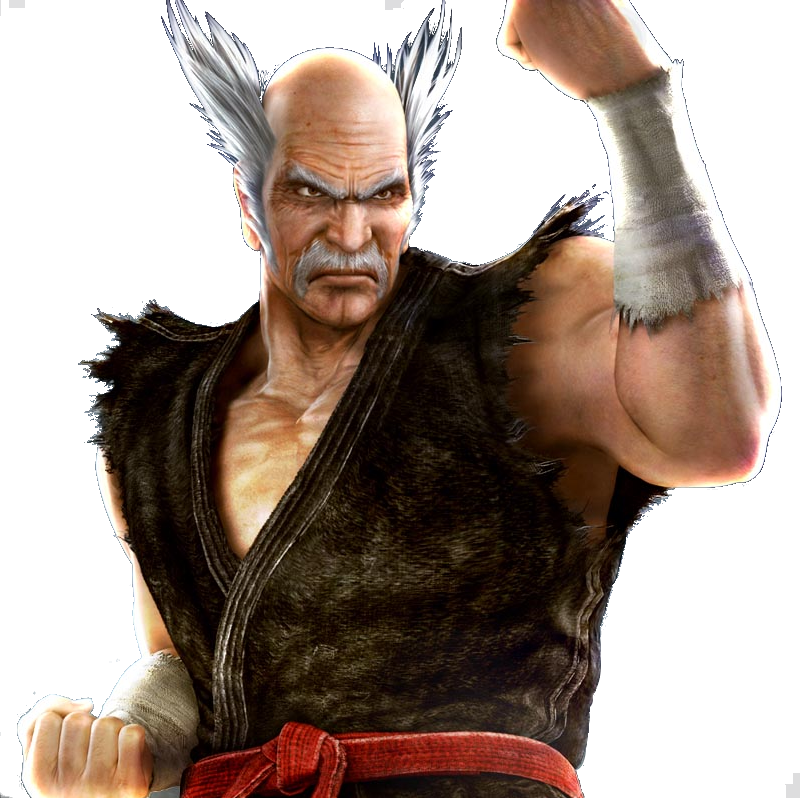
\includegraphics[height=5cm]{heihachi}
        \caption{Heihachi Mishima (Tekken 5)\footnote{\url{http://bestgamewallpapers.com/files/tekken-5/heihachi-mishima.jpg}}}
    \end{figure}
\end{frame}

% ------------------------------
\begin{frame}{\textbf{Triângulo na cabeça}}
    \centering
    \begin{figure}
        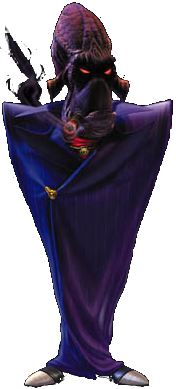
\includegraphics[height=5cm]{molluck}
        \caption{Molluck (Abe's Oddysee)\footnote{\url{http://img3.wikia.nocookie.net/__cb20090428062047/oddworld/images/c/cf/Molluck02.jpg}}}
    \end{figure}
\end{frame}


% QUADRADO
% ------------------------------
\begin{frame}{\textbf{Quadrado}}
    \centering
    \begin{figure}
        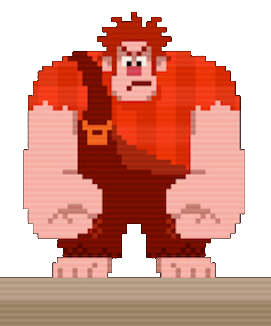
\includegraphics[height=5cm]{ralph}
        \caption{Ralph (Wreck it Ralph)\footnote{\url{http://cache.g4tv.com/ImageDb3/303386_S/wreck-it-ralph-game-coming-from-activision-and-disney-interactive.jpg}}}
    \end{figure}
\end{frame}

% ------------------------------
\begin{frame}{\textbf{Quadrado}}
    \centering
    \begin{figure}
        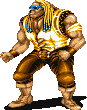
\includegraphics[height=5cm]{dammd}
        \caption{Dammd (Final Fight)\footnote{\url{http://www.arcadequartermaster.com/ffight/boss_damnd.png}}}
    \end{figure}
\end{frame}

% ------------------------------
\begin{frame}{\textbf{Quadrado}}
    \centering
    \begin{figure}
        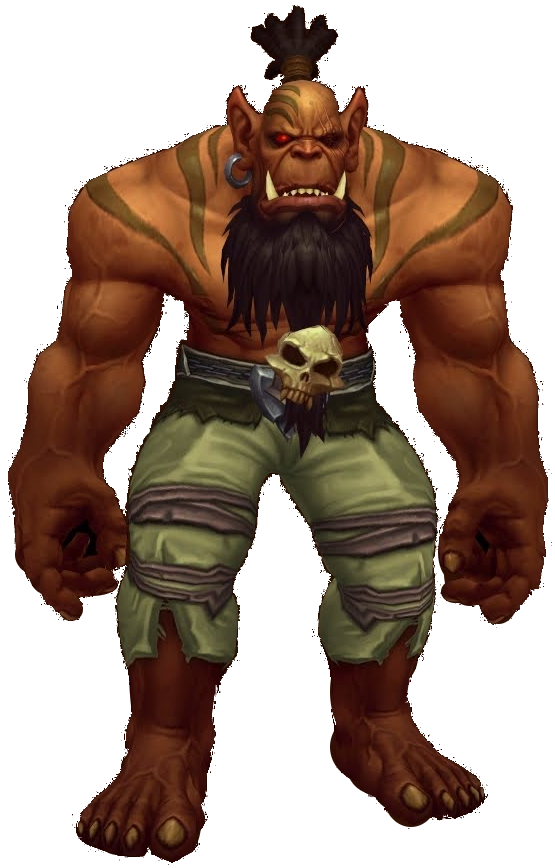
\includegraphics[height=5cm]{kilrogg}
        \caption{Kilrogg Deadeye (World of Warcraft)\footnote{\url{http://i.ytimg.com/vi/dTUIqJyy1lk/maxresdefault.jpg}}}
    \end{figure}
\end{frame}

% ------------------------------
\begin{frame}{\textbf{Quadrado}}
    \centering
    \begin{figure}
        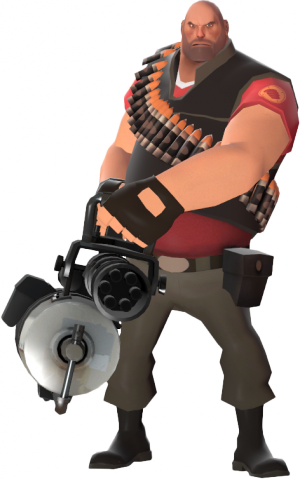
\includegraphics[height=5cm]{heavy}
        \caption{Heavy (Team Fortress 2)\footnote{\url{https://wiki.teamfortress.com/w/images/thumb/a/a0/Community_Heavy_Strategy_Header.png/300px-Community_Heavy_Strategy_Header.png?t=20111122050936}}}
    \end{figure}
\end{frame}

% ------------------------------
\begin{frame}{\textbf{Quadrado}}
    \centering
    \begin{figure}
        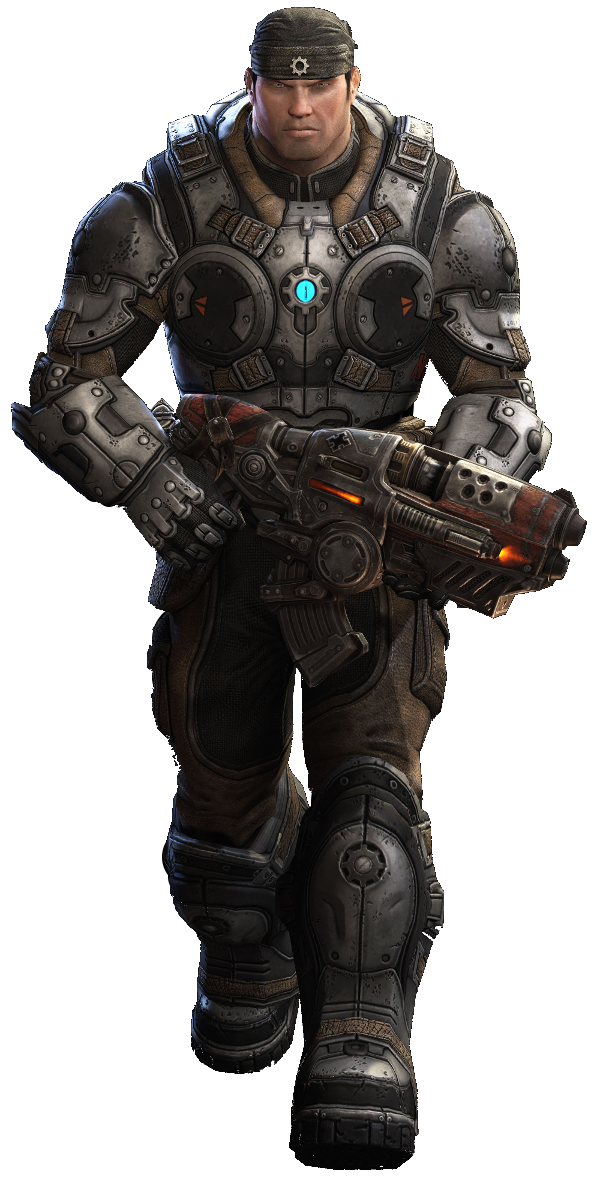
\includegraphics[height=5cm]{marcus}
        \caption{Marcus Fenix (Gears of War)\footnote{\url{http://media.gow-series.com/images/site/newsimages/gears-of-war-judgment-marcus-fenix-preorder.jpg}}}
    \end{figure}
\end{frame}


% TRIÂNGULO INVERTIDO
% ------------------------------
\begin{frame}{\textbf{Triângulo para baixo}}
    \centering
    \begin{figure}
        
\includegraphics[height=5cm]{jonny_bravo}
        \caption{Jonny Bravo\footnote{\url{http://www.jrj-socrates.com/Cartoon\%20Pics/Cartoon\%20Network/Johnny\%20Bravo/Johnny_Bravo_301.gif}}}
    \end{figure}
\end{frame}

% ------------------------------
\begin{frame}{\textbf{Triângulo para baixo}}
    \centering
    \begin{figure}
        
\includegraphics[height=5cm]{cody}
        \caption{Cody (Final Fight)\footnote{\url{http://www.arcadequartermaster.com/ffight/sprite_cody.png}}}
    \end{figure}
\end{frame}

% ------------------------------
\begin{frame}{\textbf{Triângulo para baixo}}
    \centering
    \begin{figure}
        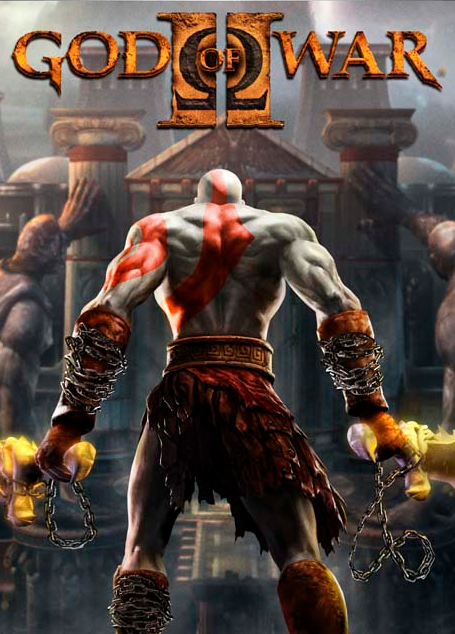
\includegraphics[height=5cm]{kratos}
        \caption{Kratos (God of War II)\footnote{\url{http://199.101.98.242/media/shots/150564-God_of_War_II_\%28USA\%29-3.jpg}}}
    \end{figure}
\end{frame}

% ------------------------------
\begin{frame}{\textbf{Triângulo para baixo}}
    \centering
    \begin{figure}
        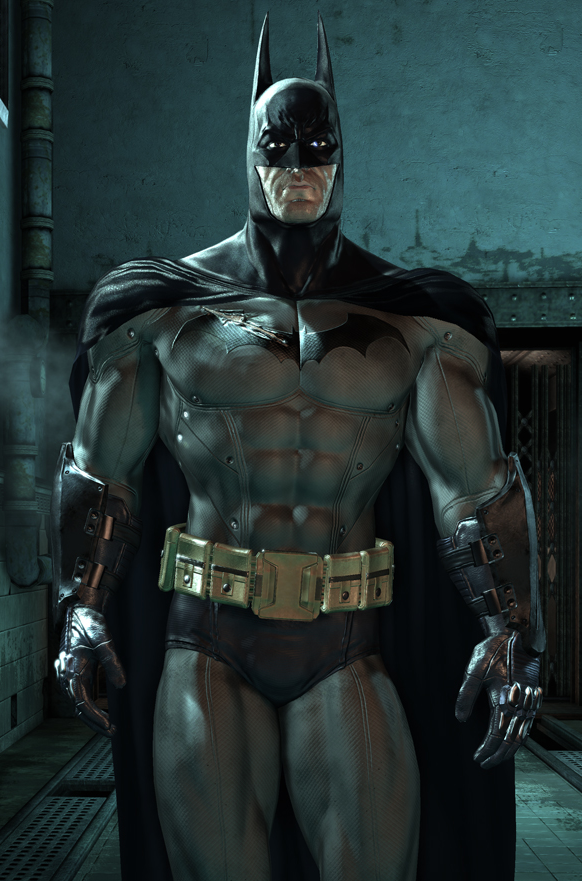
\includegraphics[height=5cm]{batman}
        \caption{Batman (Batman Arkhan Asylum)\footnote{\url{http://img1.wikia.nocookie.net/__cb20131108203507/marvel_dc/images/6/62/Batman_Arkhamverse_003.jpg}}}
    \end{figure}
\end{frame}


% Silhuetas
% ------------------------------
\begin{frame}{\textbf{Silhueta}}
    \centering
    \begin{figure}
        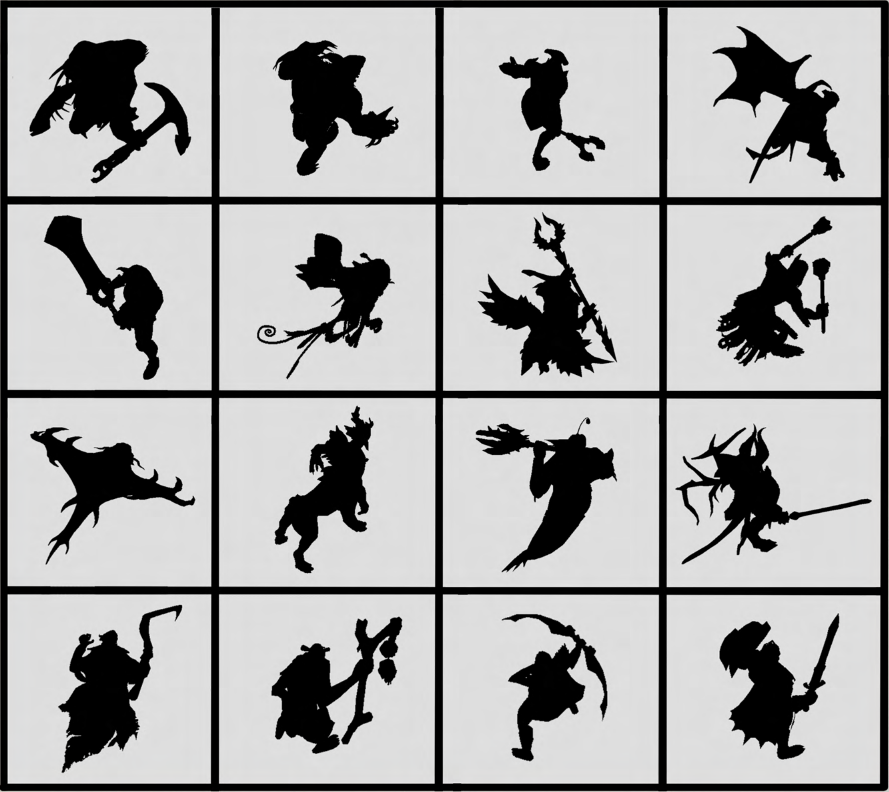
\includegraphics[height=5cm]{dota2_silhueta1}
        \caption{Dota 2 character art guide\footnote{\url{http://media.steampowered.com/apps/dota2/workshop/Dota2CharacterArtGuide.pdf}}}
    \end{figure}
\end{frame}

% ------------------------------
\begin{frame}{\textbf{Silhueta}}
    \centering
    \begin{figure}
        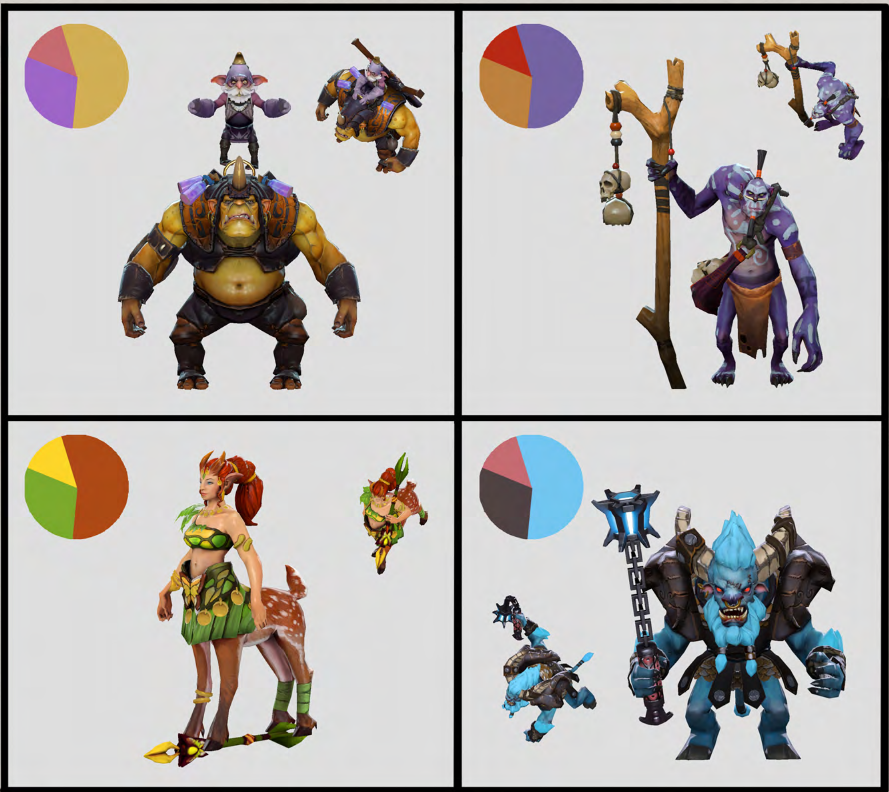
\includegraphics[height=5cm]{dota2_cores1}
        \caption{Dota 2 character art guide\footnote{\url{http://media.steampowered.com/apps/dota2/workshop/Dota2CharacterArtGuide.pdf}}}
    \end{figure}
\end{frame}

% ------------------------------
\begin{frame}{\textbf{Silhueta}}
    \centering
    \begin{figure}
        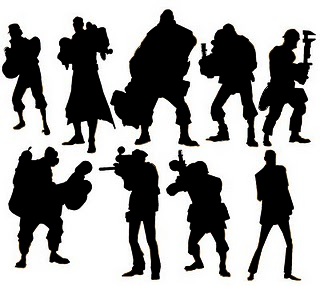
\includegraphics[height=5cm]{team_fortress2_silhueta}
        \caption{Team Fortress 2\footnote{\url{http://www.mellow3d.com/misc/tf2.png}}}
    \end{figure}
\end{frame}


% Informação pelo personagem
% ------------------------------
\begin{frame}{\textbf{O personagem mostrando informações}}
    \centering
    \begin{figure}
        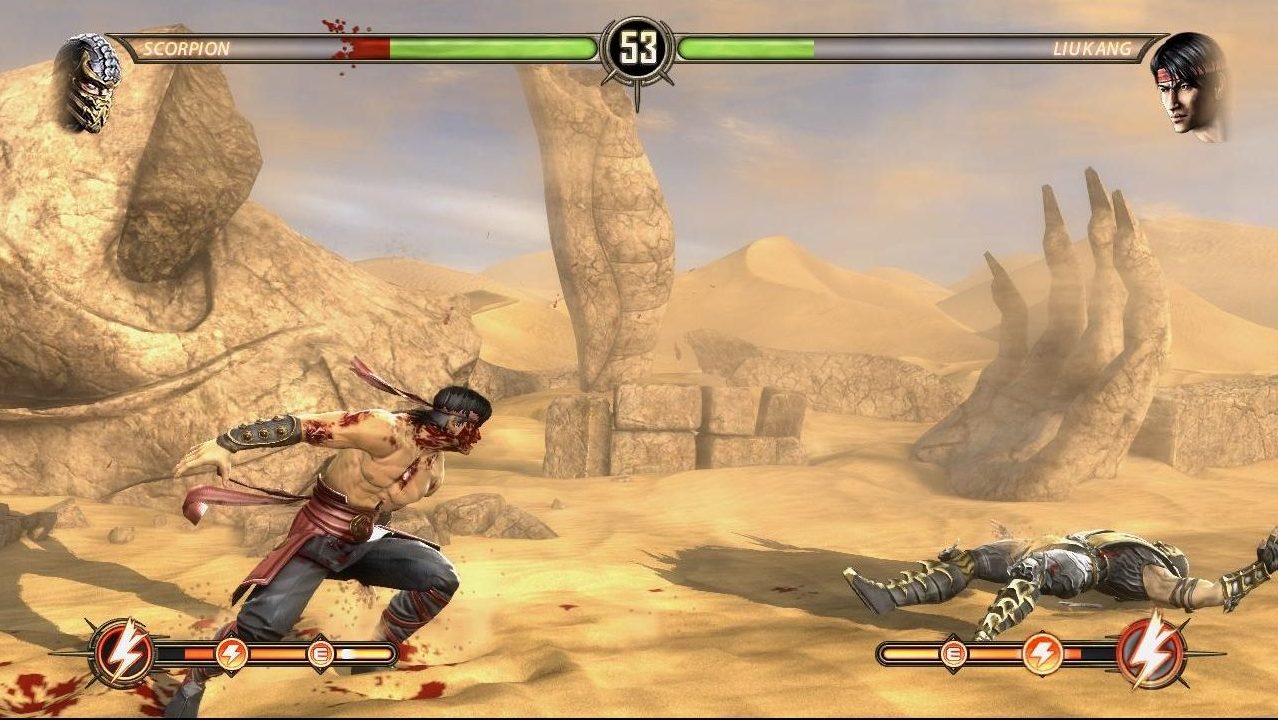
\includegraphics[height=5cm]{mk}
        \caption{Mortal Kombat 9\footnote{\url{http://i47.fastpic.ru/big/2013/0704/e5/a02c5f822d656c0c57b437b5fcc912e5.jpg}}}
    \end{figure}
\end{frame}

% ------------------------------
\begin{frame}{\textbf{O personagem mostrando informações}}
    \centering
    \begin{figure}
        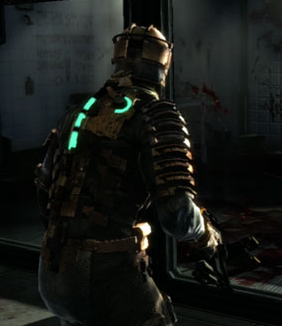
\includegraphics[height=5cm]{deadspace}
        \caption{Dead Space\footnote{\url{http://www.visualwalkthroughs.com/deadspace/intensivecare/68.jpg}}}
    \end{figure}
\end{frame}

% ------------------------------
\begin{frame}{\textbf{O personagem mostrando informações}}
    \centering
    \begin{figure}
        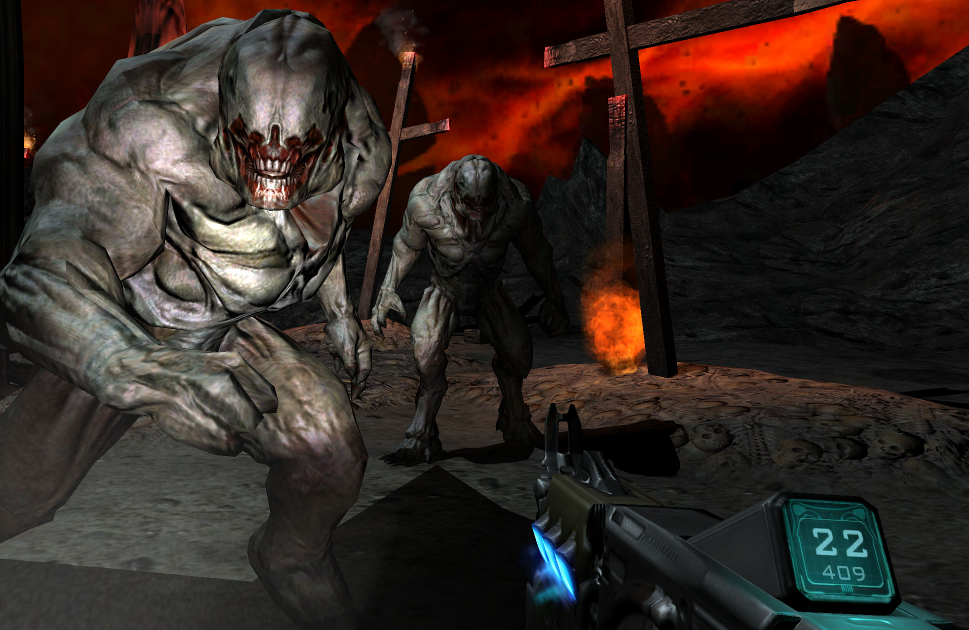
\includegraphics[height=5cm]{doom}
        \caption{Doom 3\footnote{\url{http://cdn2.gamefront.com/wp-content/uploads/2012/08/d3-1.jpeg}}}
    \end{figure}
\end{frame}


% Companheiros
% ------------------------------
\begin{frame}{\textbf{Personagens companheiros}}
    \centering
    \begin{figure}
        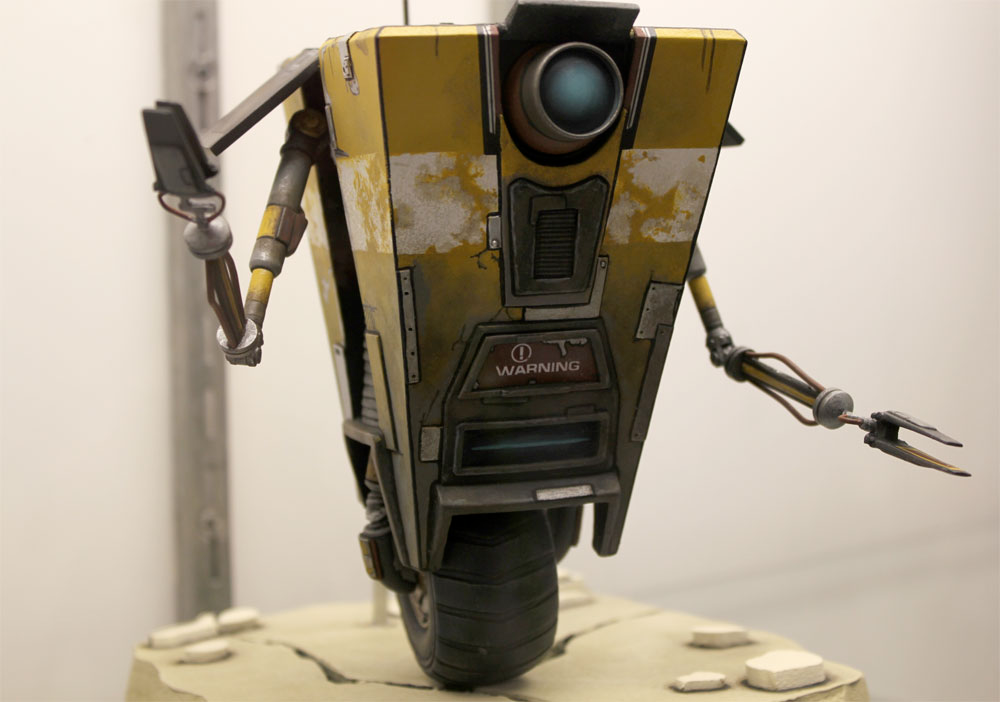
\includegraphics[height=5cm]{claptrap}
        \caption{Claptrap (Borderlands)\footnote{\url{http://i.kinja-img.com/gawker-media/image/upload/s--NHlrEvcg--/18j3aiqqtotcpjpg.jpg}}}
    \end{figure}
\end{frame}

% ------------------------------
\begin{frame}{\textbf{Personagens companheiros}}
    \centering
    \begin{figure}
        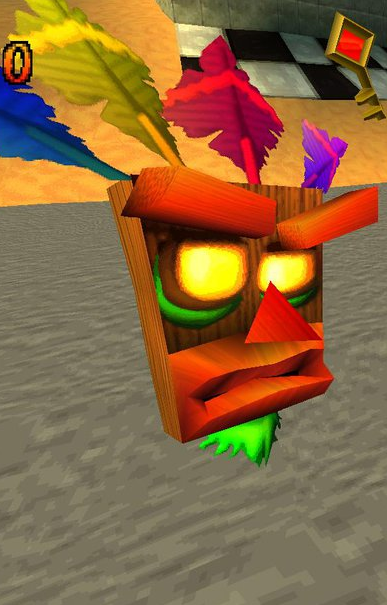
\includegraphics[height=5cm]{akuaku}
        \caption{Aku Aku (Crash Bandicoot)\footnote{\url{http://fc08.deviantart.net/fs71/i/2014/211/9/e/crash_bandicoot_team_racing_psx_aku_aku_by_danytatu-d7sxgo7.jpg}}}
    \end{figure}
\end{frame}

% -
% ------------------------------
\begin{frame}{\textbf{Personagens companheiros}}
    \centering
    \begin{figure}
        
\includegraphics[height=5cm]{sonic_tails}
        \caption{Tails (Sonic the Hedgehog 2)\footnote{\url{http://img1.wikia.nocookie.net/__cb20091012201501/sonic/images/4/49/Sonic_and_Tails_5.png}}}
    \end{figure}
\end{frame}

% ------------------------------
\begin{frame}{\textbf{Personagens companheiros}}
    \centering
    \begin{figure}
        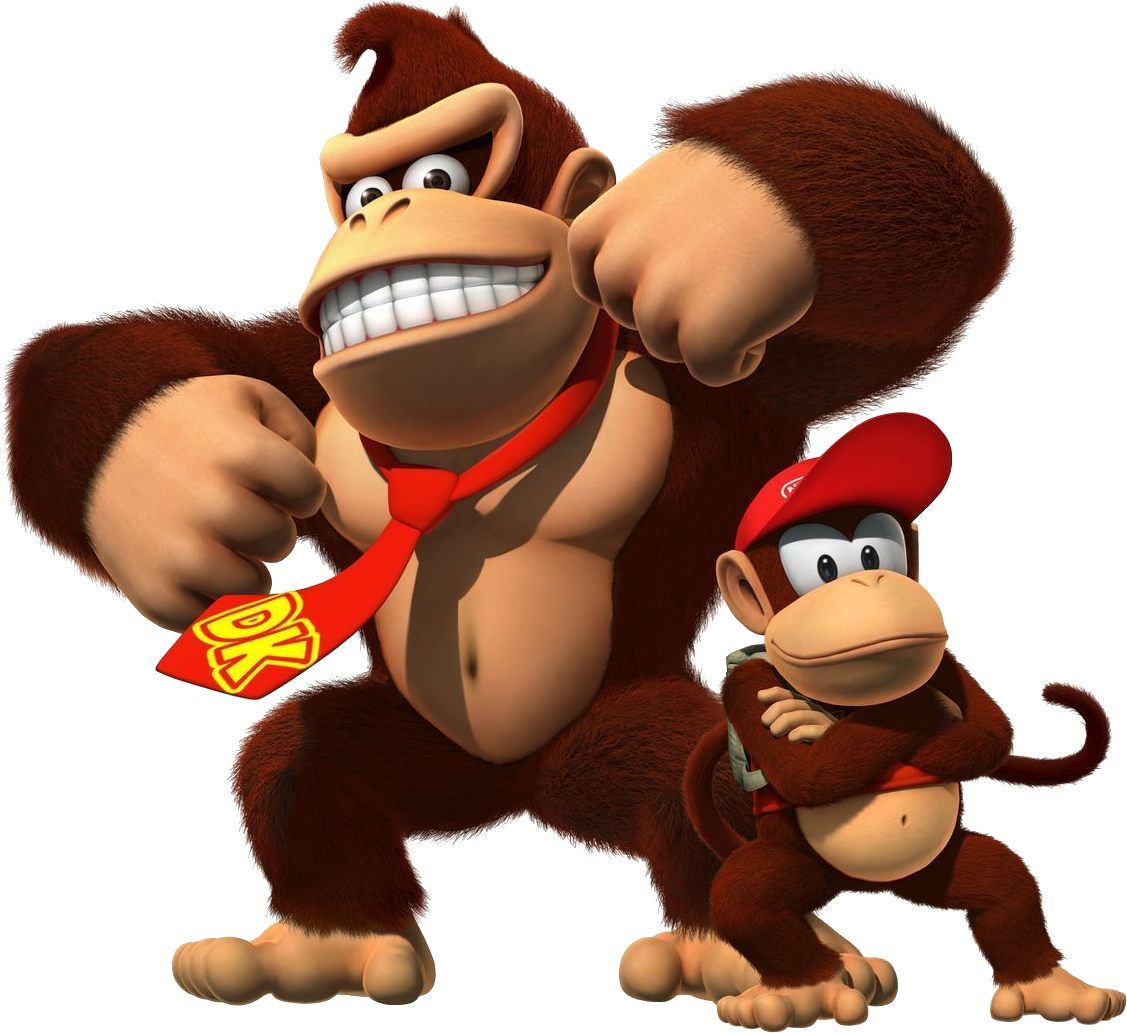
\includegraphics[height=5cm]{donkey_diddy}
        \caption{Diddy (Donkey Kong Country)\footnote{\url{http://images4.fanpop.com/image/photos/22000000/Donkey-and-Diddy-Kong-donkey-kong-22009280-1280-1280.jpg}}}
    \end{figure}
\end{frame}

% ------------------------------
\begin{frame}{\textbf{Personagens companheiros}}
    \centering
    \begin{figure}
        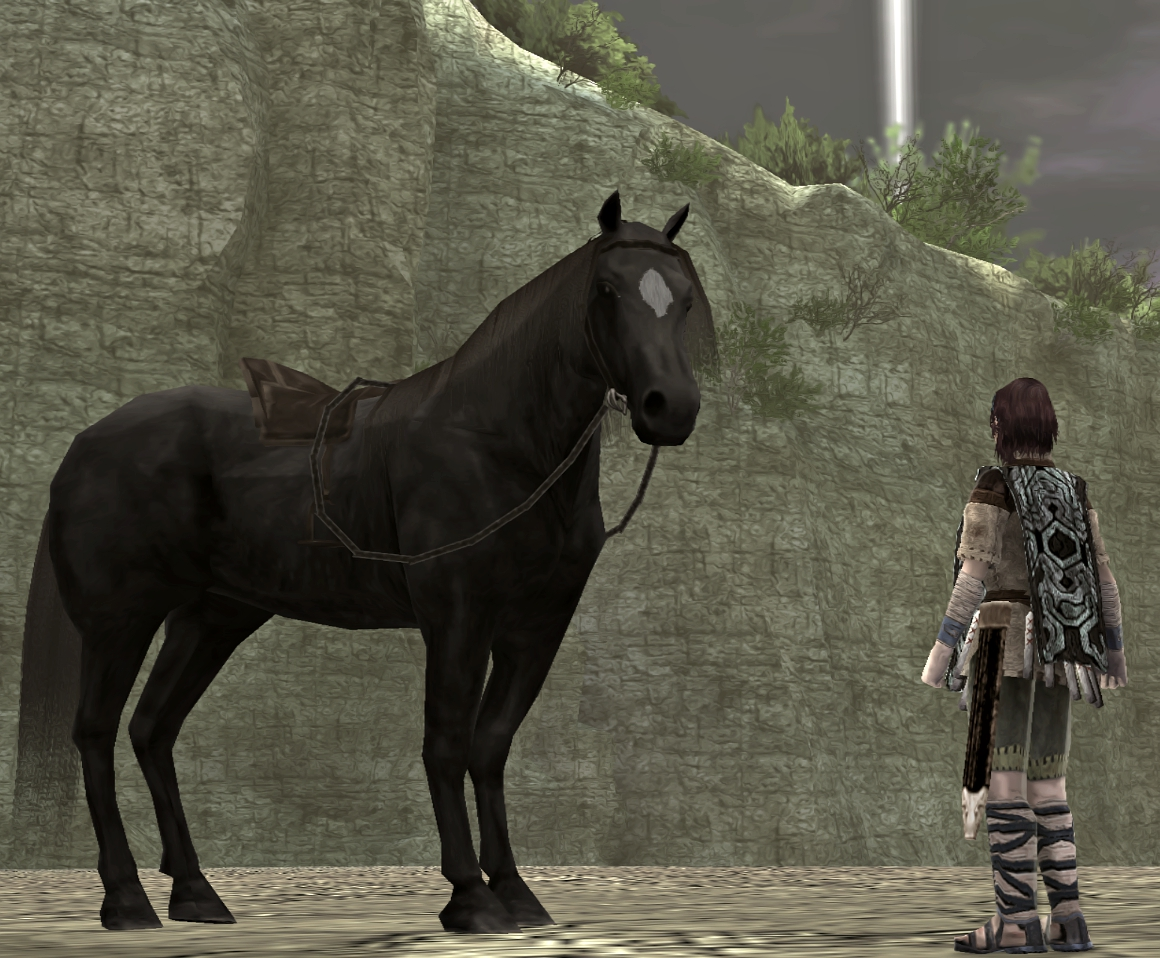
\includegraphics[height=5cm]{agro}
        \caption{Agro (Shadow of the Colossus)\footnote{\url{http://moderatelygeeky.com/wp-content/uploads/2013/12/Agro.jpg}}}
    \end{figure}
\end{frame}


% Dimensões
% ------------------------------
\begin{frame}{\textbf{Personagens como unidade de medida}}
    \centering
    \begin{figure}
        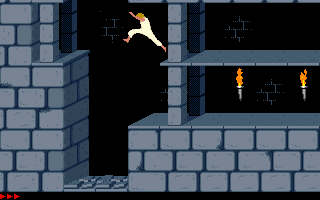
\includegraphics[height=5cm]{prince_of_persia}
        \caption{Prince of Persia\footnote{\url{http://www.popuw.com/images/pop1-16.png}}}
    \end{figure}
\end{frame}



% ------------------------------
\subsection{Câmera}

% Fixa
% ------------------------------
\begin{frame}{\textbf{Câmera fixa}}
    \centering
    \begin{figure}
        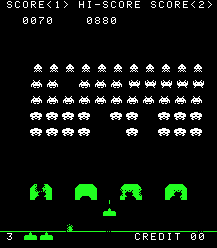
\includegraphics[height=5cm]{space_invaders}
        \caption{Space Invaders\footnote{\url{http://upload.wikimedia.org/wikipedia/en/2/20/SpaceInvaders-Gameplay.gif}}}
    \end{figure}
\end{frame}

%Fear Effect
%http://mlb-s2-p.mlstatic.com/fear-effect-1-playstation-1-psx-4-discos-frete-gratis-16612-MLB20124183563_072014-F.jpg
%http://www.theisozone.com/images/screens/playstation-57563-41409572983.jpg
%http://s.uvlist.net/l/y2006/09/26654.jpg
%fear_effect1.png
%fear_effect3.png
%fear_effect2.png

% Rolagem
% ------------------------------
\begin{frame}{\textbf{Câmera de rolagem}}
    \centering
    \begin{figure}
        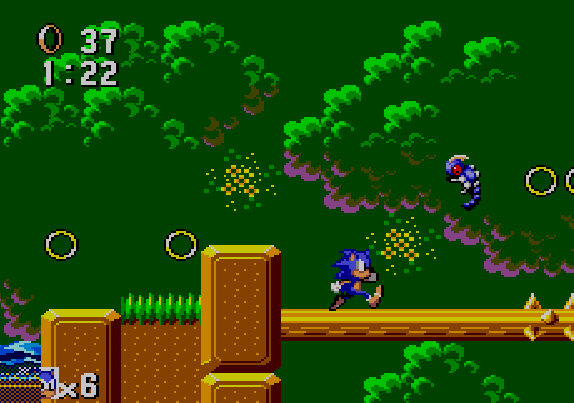
\includegraphics[height=5cm]{sonic_screenshot}
        \caption{Sonic the hedhog\footnote{\url{http://3.bp.blogspot.com/_WaXspDnBJ2c/TC1lZyJEZqI/AAAAAAAACrg/KtPBQA1X3FI/s1600/02.png}}}
    \end{figure}
\end{frame}

% ------------------------------
\begin{frame}{\textbf{Câmera de rolagem}}
    \centering
    \begin{figure}
        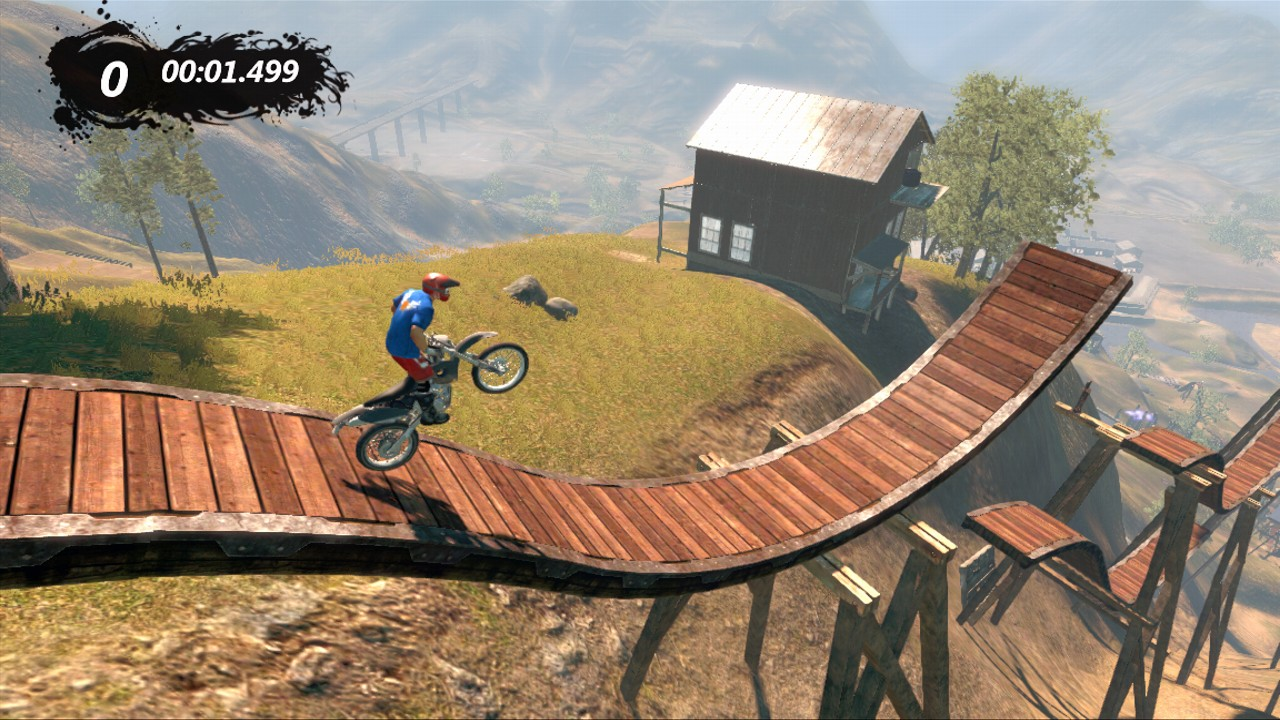
\includegraphics[height=5cm]{trials_evolution}
        \caption{Trials Evolution\footnote{\url{http://www.redlynx.com//images/stories/games/trialsevo/screenshots2/trials-evo-010.jpg}}}
    \end{figure}
\end{frame}

% Primeira pessoa
% ------------------------------
\begin{frame}{\textbf{Câmera em primeira pessoa}}
    \centering
    \begin{figure}
        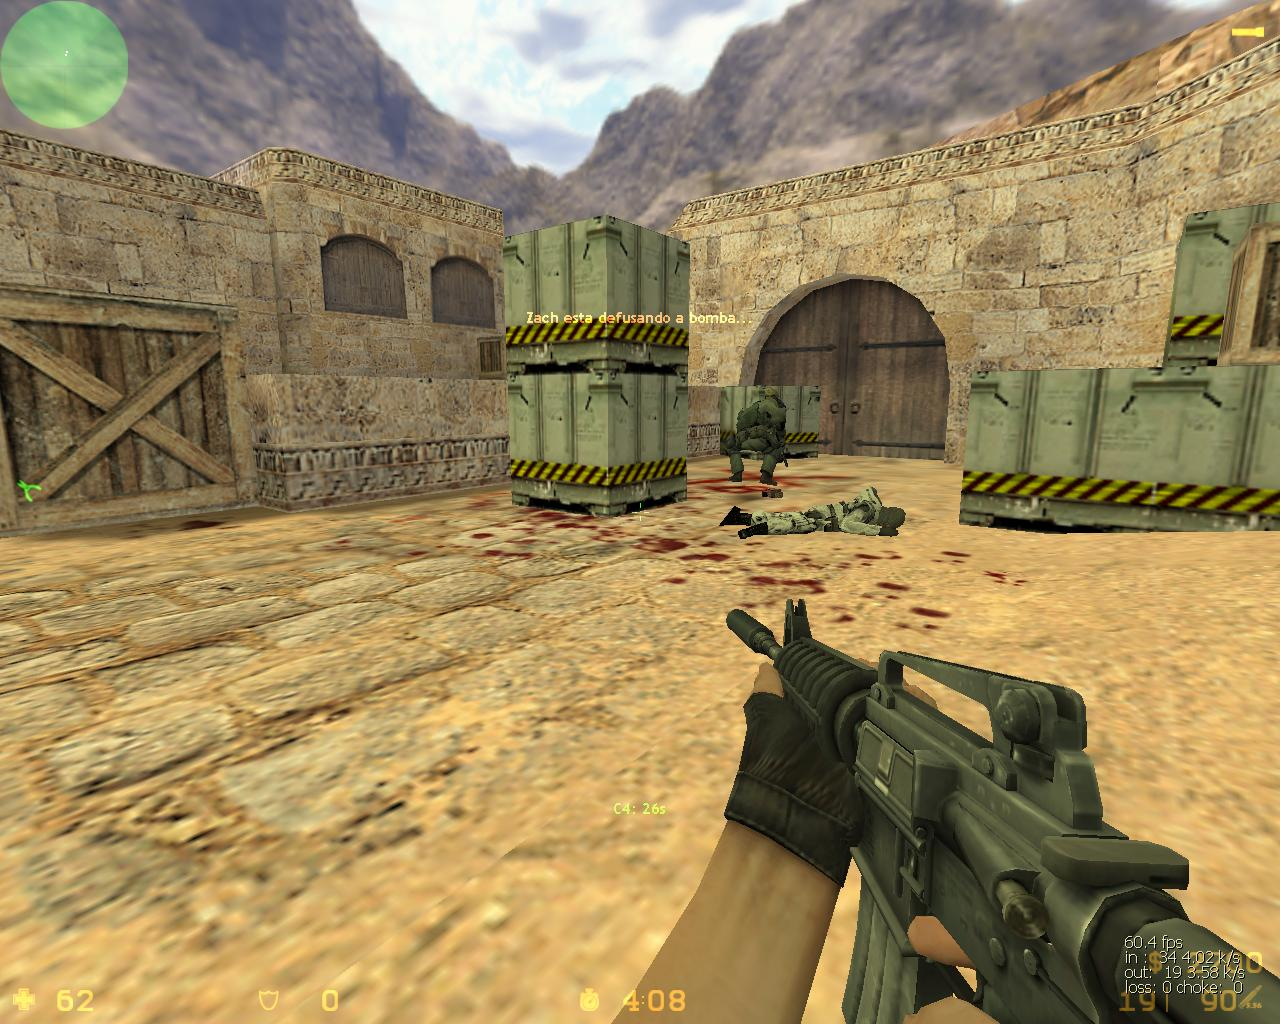
\includegraphics[height=5cm]{cs}
        \caption{Counter Strike\footnote{\url{http://www.hivegaming.net/images/cs16-screencaps/large/01.jpg}}}
    \end{figure}
\end{frame}

% ------------------------------
\begin{frame}{\textbf{Câmera em primeira pessoa}}
    \centering
    \begin{figure}
        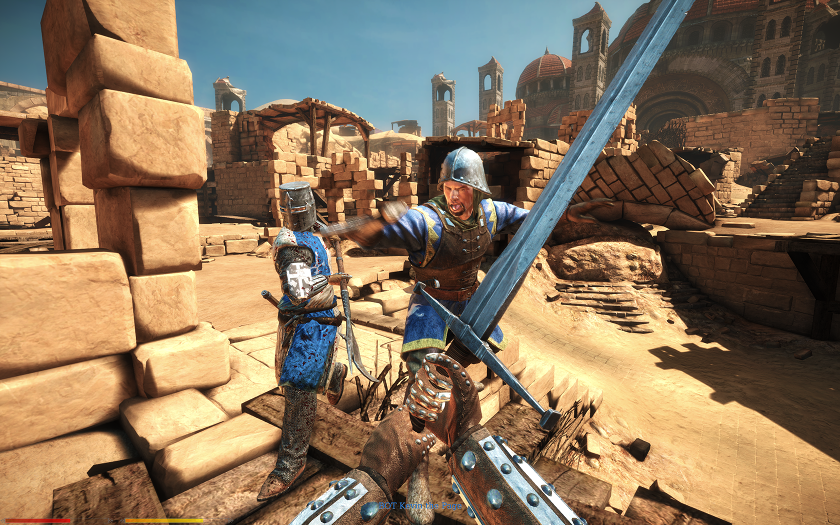
\includegraphics[height=5cm]{chivalry}
        \caption{Chivalry Medieval Warfare\footnote{\url{http://vignette2.wikia.nocookie.net/age-of-chivalry/images/f/fa/I9dNyaRha8FpE_\%281\%29.png/revision/latest?cb=20121215022358}}}
    \end{figure}
\end{frame}

% ------------------------------
\begin{frame}{\textbf{Câmera em primeira pessoa}}
    \centering
    \begin{figure}
        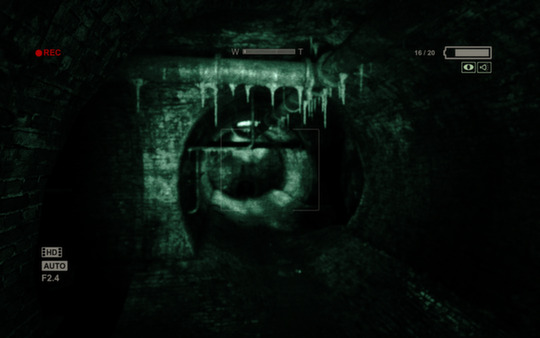
\includegraphics[height=5cm]{outlast}
        \caption{Outlast\footnote{\url{http://cdn.akamai.steamstatic.com/steam/apps/238320/ss_97dfd31784f9c51d2c603ac3f36ae52fac401de3.600x338.jpg?t=1399595107}}}
    \end{figure}
\end{frame}

% ------------------------------
\begin{frame}{\textbf{Câmera em primeira pessoa}}
    \centering
    \begin{figure}
        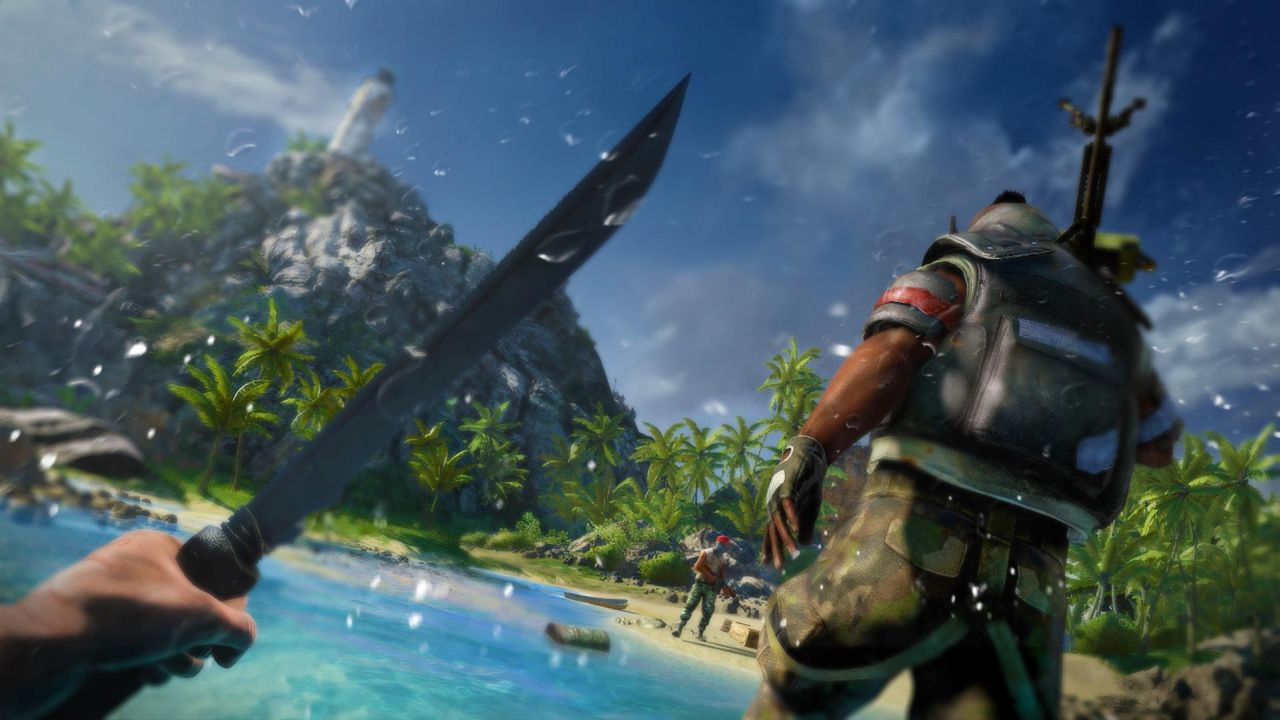
\includegraphics[height=5cm]{farcry3_drops}
        \caption{Far Cry 3\footnote{\url{http://gamingsnack.com/wp-content/uploads/2013/01/Far-Cry-3-PS3.jpg}}}
    \end{figure}
\end{frame}

% Terceira pessoa
% ------------------------------
\begin{frame}{\textbf{Câmera em terceira}}
    \centering
    \begin{figure}
        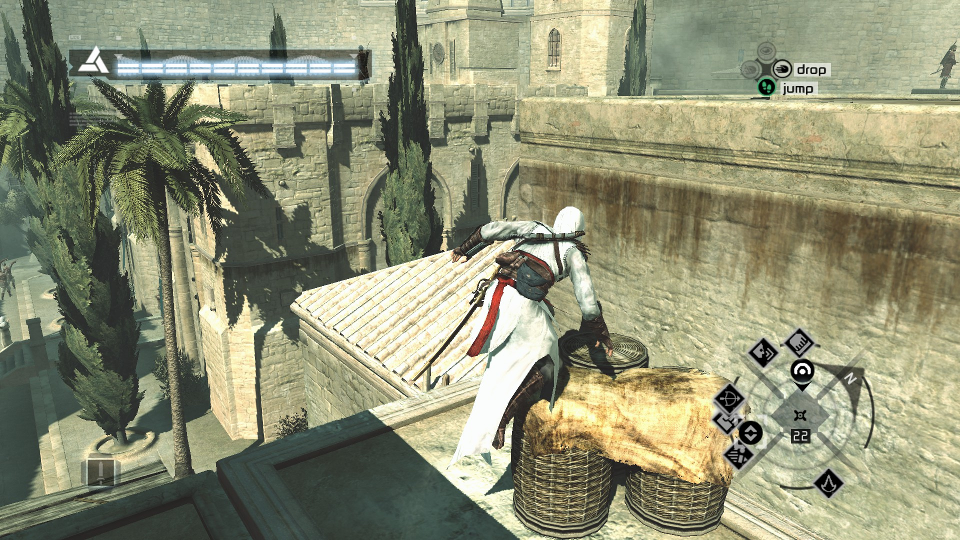
\includegraphics[height=5cm]{assassins_creed}
        \caption{Assassin's Creed\footnote{\url{http://blog.gaming.stackexchange.com/files/2011/06/acreed_03.jpg}}}
    \end{figure}
\end{frame}

% ------------------------------
\begin{frame}{\textbf{Câmera em terceira}}
    \centering
    \begin{figure}
        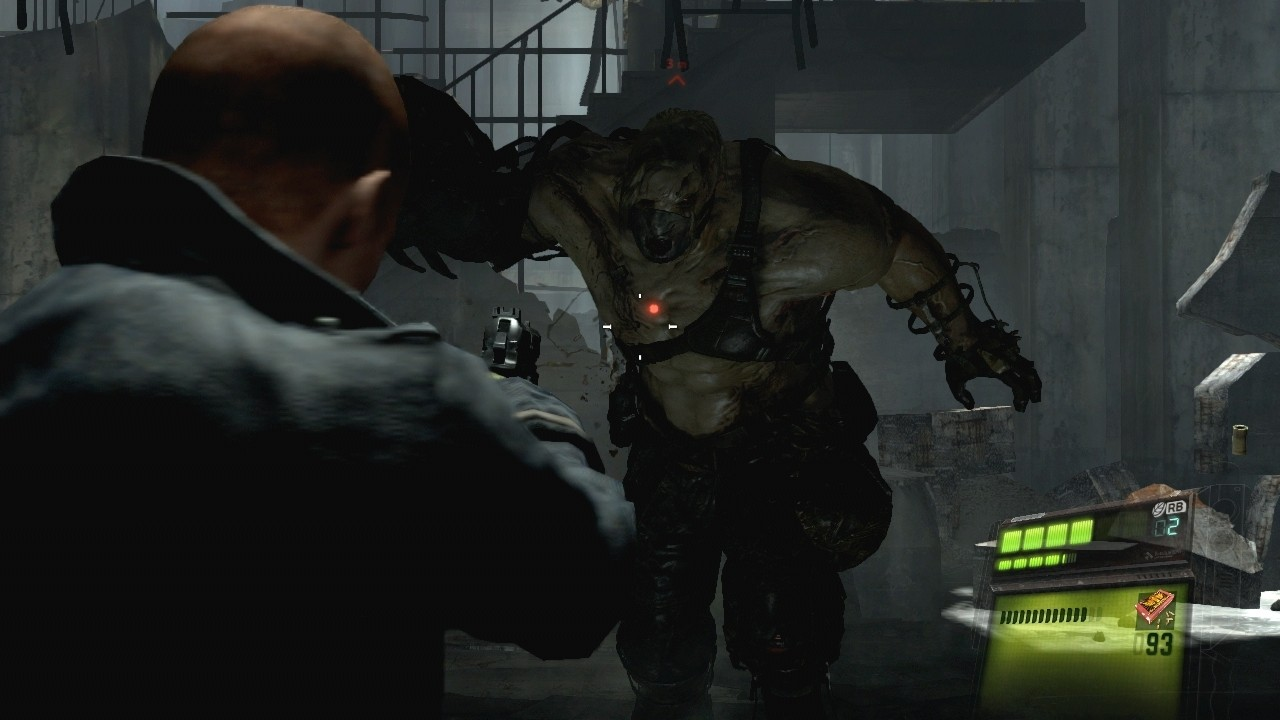
\includegraphics[height=5cm]{resident_evil6}
        \caption{Resident Evil 6\footnote{\url{http://gamehall.uol.com.br/selectgame/wp-content/gallery/resident-evil-6-1/resident-evil-6-gameplay-7.jpg}}}
    \end{figure}
\end{frame}

% 2.5D
% ------------------------------
\begin{frame}{\textbf{2.5D}}
    \centering
    \begin{figure}
        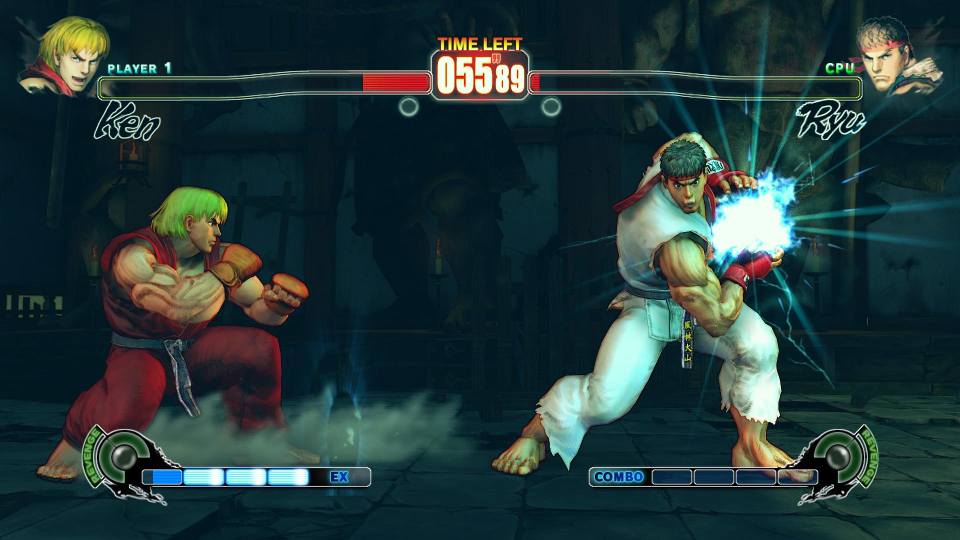
\includegraphics[height=5cm]{street_fighter}
        \caption{Street Fighter IV\footnote{\url{http://ha.wishmesh.com/wp-content/uploads/2011/04/street-fighter-iv-ken-vs-ryu.jpg}}}
    \end{figure}
\end{frame}

% ------------------------------
\begin{frame}{\textbf{2.5D}}
    \centering
    \begin{figure}
        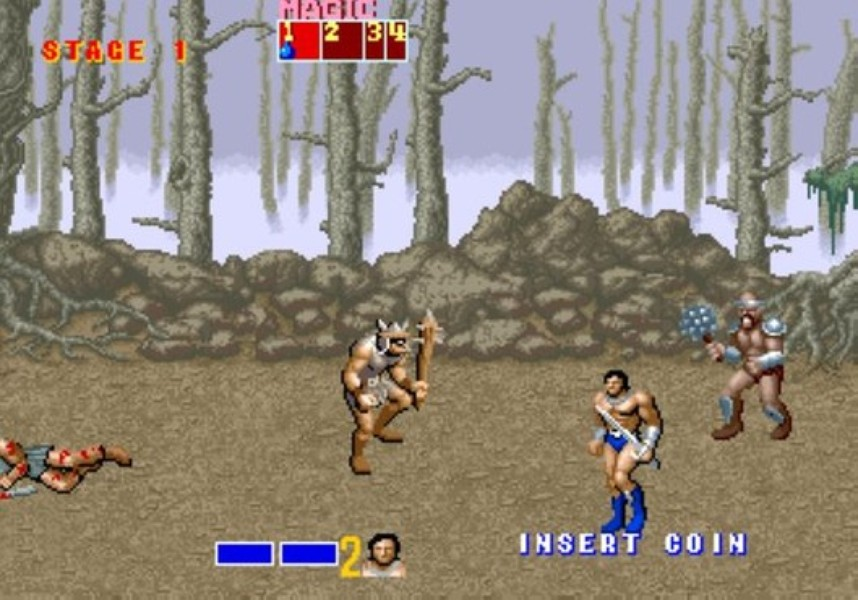
\includegraphics[height=5cm]{golden_axe}
        \caption{Golden Axe\footnote{\url{http://s2.glbimg.com/VWgbIztytg3JVLUQdEwLGATYPMk=/0x600/s.glbimg.com/po/tt2/f/original/2014/09/11/a450e98e012c44fd12313b030e0a.jpeg}}}
    \end{figure}
\end{frame}

% Isométrica
% ------------------------------
\begin{frame}{\textbf{Projeção isométrica}}
    \centering
    \begin{figure}
        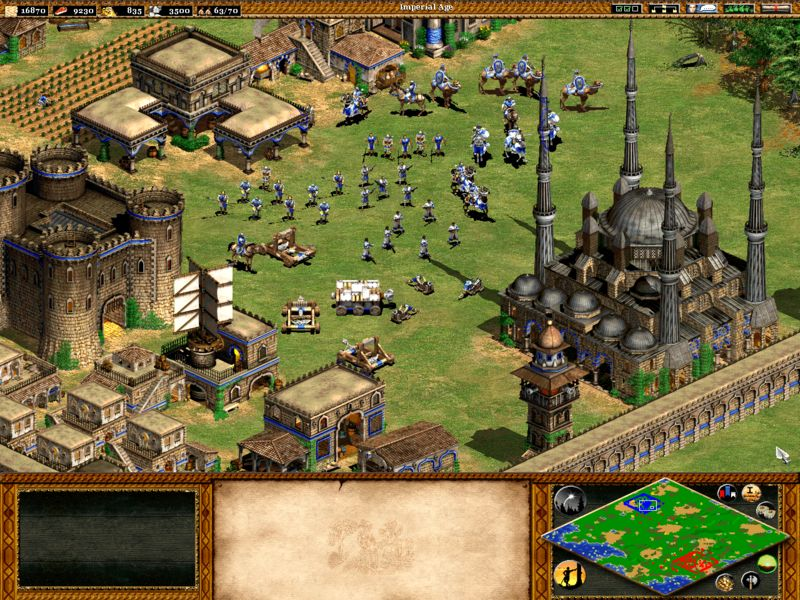
\includegraphics[height=5cm]{age_of_empires2}
        \caption{Age of Empires II\footnote{\url{http://www.infobarrel.com/media/image/137340.jpg}}}
    \end{figure}
\end{frame}


% ------------------------------
\subsection{Controle}

% ------------------------------
\begin{frame}{\textbf{Controle}}

%http://www.wintecind.com/features/filemate/imagegallery/Notebook/images/B2020/3FMNB2020WBK-R_800953176162_AV.jpg
%keyboard.png

%http://images.amazon.com/images/G/01/videogames/detail-page/B000IMYKQ0-1-lg.jpg
%wii_controller.png

%http://pixabay.com/get/b3d60eb87415c735405c/1420749677/tablet-314153_1280.png?direct
%touch.png

%http://www.evilcontrollers.com/media/catalog/product/cache/1/image/490x351/9df78eab33525d08d6e5fb8d27136e95/x/b/xboxone-frontview-stockblack.png
%xbox_cotroller.png

%http://ecx.images-amazon.com/images/I/71uQYNKiKCL._SL1500_.jpg
%playstation_controller.png
\end{frame}

% Ergonomia
% ------------------------------
\begin{frame}{\textbf{Controle}}
Level UP! - Scott Rogers
ergonomia.png
\end{frame}


% ---------------------------------------------------------------------------- %
\section{Jogabilidade}
% ---------------------------------------------------------------------------- %

% ------------------------------
\subsection{Protejendo o jogador de erros} %...e ajudando-o a corrigí-los
    % -> Save points
    % -> Guiar o jogador (Regra do olho espremido)
    % -> Bloquear acesso a áreas erradas
    % -> NPC’s de auxílio (tanto físico como de orientação geral)

% ------------------------------
\subsection{Consistência}
    % -> as ações têm sempre o mesmo efeito
    % -> o avatar é capaz de nadar ou não (ou toda água mata)

% ------------------------------
\subsection{Sequência lógica de desafios}
    % -> Balanceamento de dificuldades


% ---------------------------------------------------------------------------- %
\section{Gráfico de ritmo}
% ---------------------------------------------------------------------------- %

% ------------------------------
\begin{frame}{\textbf{Gráfico de ritmo}}
    \centering
    Na verdade não é um gráfico...
    \vskip 2em

    são tabelas.
\end{frame}

% ------------------------------
\begin{frame}{\textbf{Gráfico de ritmo}}
    \centering
    \begin{minipage}{7cm}
        \begin{itemize}
            \item Descrição sussinta de cada fase
            \vskip 0.3cm%
            \item Permite acompanhar e controlar...
            \begin{itemize}
                \item aparecimento de inimigos novos
                \item aprendizado de novas habilidades
                \item surgimento de novas mecânicas
                \item dinheiro do personagem
                \item etc
            \end{itemize}
            \vskip 0.3cm%
            \item Muito útil para balanceamento
        \end{itemize}
    \end{minipage}
\end{frame}

% ------------------------------
\begin{frame}{\textbf{Gráfico de ritmo}}
    \scriptsize
    \begin{table}[h]
    \begin{tabular}{l p{6cm}}
    \hline
    \textbf{Número do nível}         & 1.2                             \\ \hline
    \textbf{Título/ambiente}         & Tumba dos escravos              \\ \hline
    \textbf{Hora do dia}             & Noite                           \\ \hline
    \textbf{Elementos de história}   & Kha encontra um mapa e sai da pimâmide
                                       por uma passagem secreta feita pelos
                                       escravos                        \\ \hline
    \textbf{Progressão de gameplay}  & Jogador sabe se movimentar e combate
                                       básico                          \\ \hline
    \textbf{Inimigos}                & Escaravelhos rastejantes, escaravelhos
                                       voadores, múmias de escravos (básico),
                                       múmias de escravos (com ferramentas)
                                       \\ \hline
    \textbf{Mecânicas}               & Alavancas, portas escondidas, vazos
                                       quebráveis, plataformas móveis, escritas
                                       nas paredes                     \\ \hline
    \textbf{Perigos}                 & Armadilha de espinhos na parede,
                                       alçapões, lâminas caindo, abismos
                                       \\ \hline
    \textbf{Tempo para completar}    & 15 minutos                      \\ \hline
    \textbf{Habilidades destravados} & Olhar item de perto, pulo duplo,
                                       escorregar                      \\ \hline
    \textbf{Power-ups encontrados}   & Haste de alavanca, recuperar vida,
                                       vagalume, moedas de ouro, moedas de prata
                                       \\ \hline
    \textbf{Tesouros}                & 25 moedas de prata, 5 moedas de ouro
                                       \\ \hline
    \textbf{Esquema de cores}        & Bege (paredes), marrom (terra/chão),
                                       dourado (estátuas)              \\ \hline
    \textbf{Trilha musical}          & lento\_mistério                 \\ \hline
    \textbf{Material extra}          & -                               \\ \hline
    \end{tabular}
    \end{table}
\end{frame}


% ---------------------------------------------------------------------------- %
\section{Átomos de jogos}
% ---------------------------------------------------------------------------- %

% ------------------------------
\begin{frame}{\textbf{Átomos de jogos}}
    \centering
    \footnotesize
    \begin{minipage}{7cm}
        \begin{itemize}
            \item Objetivo Claro
            \item Recompensas e punições
            \item Jogador como Agente de Mudança
            \item Contexto Compreensível (* rever o que é)
            \item Regras Compreensíveis
            \item Habilidade e Progressão
            \item Feedback sobre resultado (visual ou sonoro)
            \item Interface consistente
            \item Desafios e IA (desafios tipo "soma zero", mesmo sem oponentes
                  humanos)
            \item Alternância entre Desafios e Pausas
            \item Balanceamento entre sorte e estratégia
                  %(sem demonizar os extremos - jogo da vida x xadrez)
            \item Visibilidade e localização/orientação
            \item Uso de padrões
            \item Narrativa e fantasia significativas
        \end{itemize}
    \end{minipage}
\end{frame}


% ---------------------------------------------------------------------------- %
\section{Atividade}
% ---------------------------------------------------------------------------- %

% ------------------------------
\begin{frame}{Atividade}
    \centering
    \begin{minipage}{6cm}
        \begin{itemize}
            \item Analisar o balanceamento e ritmo do gameplay do projeto
            \vskip 1cm%
            \item Atualizar o GDD do projeto conforme o necessário
        \end{itemize}
	\end{minipage}
\end{frame}

\end{document}

